\subsection{Background}
Virtual Reality (VR) technology is an area of wearables that have been on the rise
as computer hardware capabilities improve. The Virtual Reality Society defines VR as
a 3D environment generated by a computer that a person can interact with, and be
immersed in such a way that the person can manipulate and interact with the environment
much like they would in \textit{actual} reality \cite{vr_soc_defn}. High-quality
technology and intelligent architectures are required to realize VR due to
the compute-intensive task of processing many inputs and rendering a virtual
world/environment in real time, and depending on the level of detail (LoD), is
an intensive task on its own \cite{hickey_wt4_pres}. Therefore, it is necessary
to make intelligent architecture design decisions to ensure the VR wearable operates
as intended, and with the correct performance specifications.

The most common type of VR wearable is the VR headset, and example is shown below in
Figure \ref{vr:example}. As illustrated, the headset is worn on the head (making it
a wearable), and its screen takes up the user's entire field of view - thereby immersing
them in a virtual environment. Some headsets include audio capabilities and movement
sensors, but this will be discussed later in this section.


\begin{figure}[h]
    \centering
    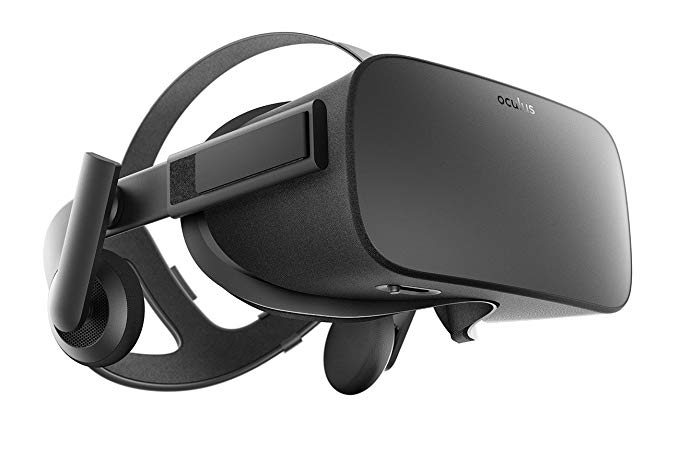
\includegraphics[width=.3\linewidth]{media/vr_headset_example.jpg}
    \caption{Example of a typical VR headset \cite{vr_headset_pic}}
    \label{vr:example}
\end{figure}

\subsection{Typical Use Cases}
Due to the immersive and potentially high-fidelity rendering that VR can accomplish,
there are several key applications where this technology can be applied. For example, 
VR has enormous potential for entertainment, business, and medical applications.

\subsubsection{Entertainment}
For entertainment applications, VR has the potential to revolutionize video games.
VR offers the ultimate level of immersion, and allows players to feel as if they
are a part of the world in which they are playing, as shown below in Figure \ref{vr:saber}
with a game called Beat Saber.
Different VR technologies offer additional peripherals, which can include treadmill-like
surfaces to track players' movements in-game, and controllers
shaped like gloves that offer haptic feedback when players interact with objects in-game,
thereby taking away elements that limit the immersion of video games \cite{vr_peripherals}.

\begin{figure}[h]
    \centering
    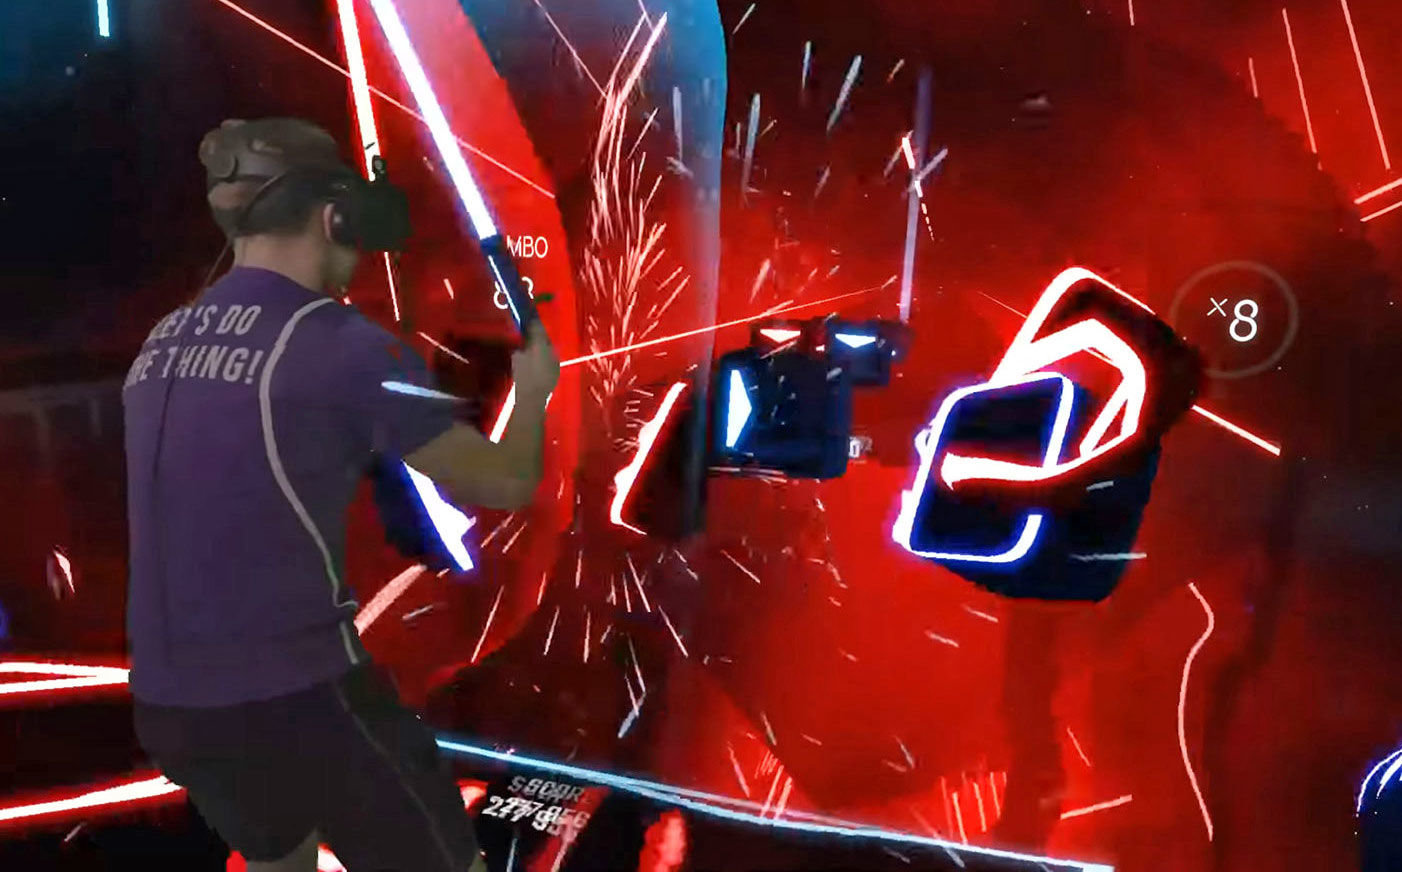
\includegraphics[width=.5\linewidth]{media/beatsaber_vr.jpg}
    \caption{Playing a video game in VR \cite{beatsaber_cite}}
    \label{vr:saber}
\end{figure}

\subsubsection{Business}
For business applications, VR can be used for modelling buildings before they break
ground, but also for completing expensive and dangerous training exercises at a lower
cost, and with zero risk. ExxonMobil has started doing this recently.
Exxon's VR simulator is quite advanced, letting users manipulate the 
virtual world by tracking their head, arm, and leg movements to allow them to 
complete virtual training work on a 3D model of one of Exxon's real assets \cite{exxon_vr}.
Exxon's VR training setup is shown below in Figure \ref{vr:exxon}.
This allows extensive training to be completed with zero consequence of failure and
without having the need to actually send trainees to the asset, saving the company money.

\begin{figure}[h]
    \centering
    \includegraphics[width=.5\linewidth]{media/exxon_vr.jpg}
    \caption{An ExxonMobil employee trains using VR \cite{exxon_vr}}
    \label{vr:exxon}
\end{figure}

\subsubsection{Medical}
For medical applications, VR can be used as both a training tool (shown in
Figure \ref{vr:med_train}), and can allow the realization of telepresence 
surgery, where a surgeon can operate on a patient through virtual reality 
from a remote site, while complex machines follow the surgeon's actions 
with acute precision \cite{vr_med_app}. This can allow doctors to receive
life-like training without having patients going under the knife, and will allow
patients requiring surgery in remote locations to have specialized surgery without the
presence of a specialized surgeon.

\begin{figure}[h!]
    \centering
    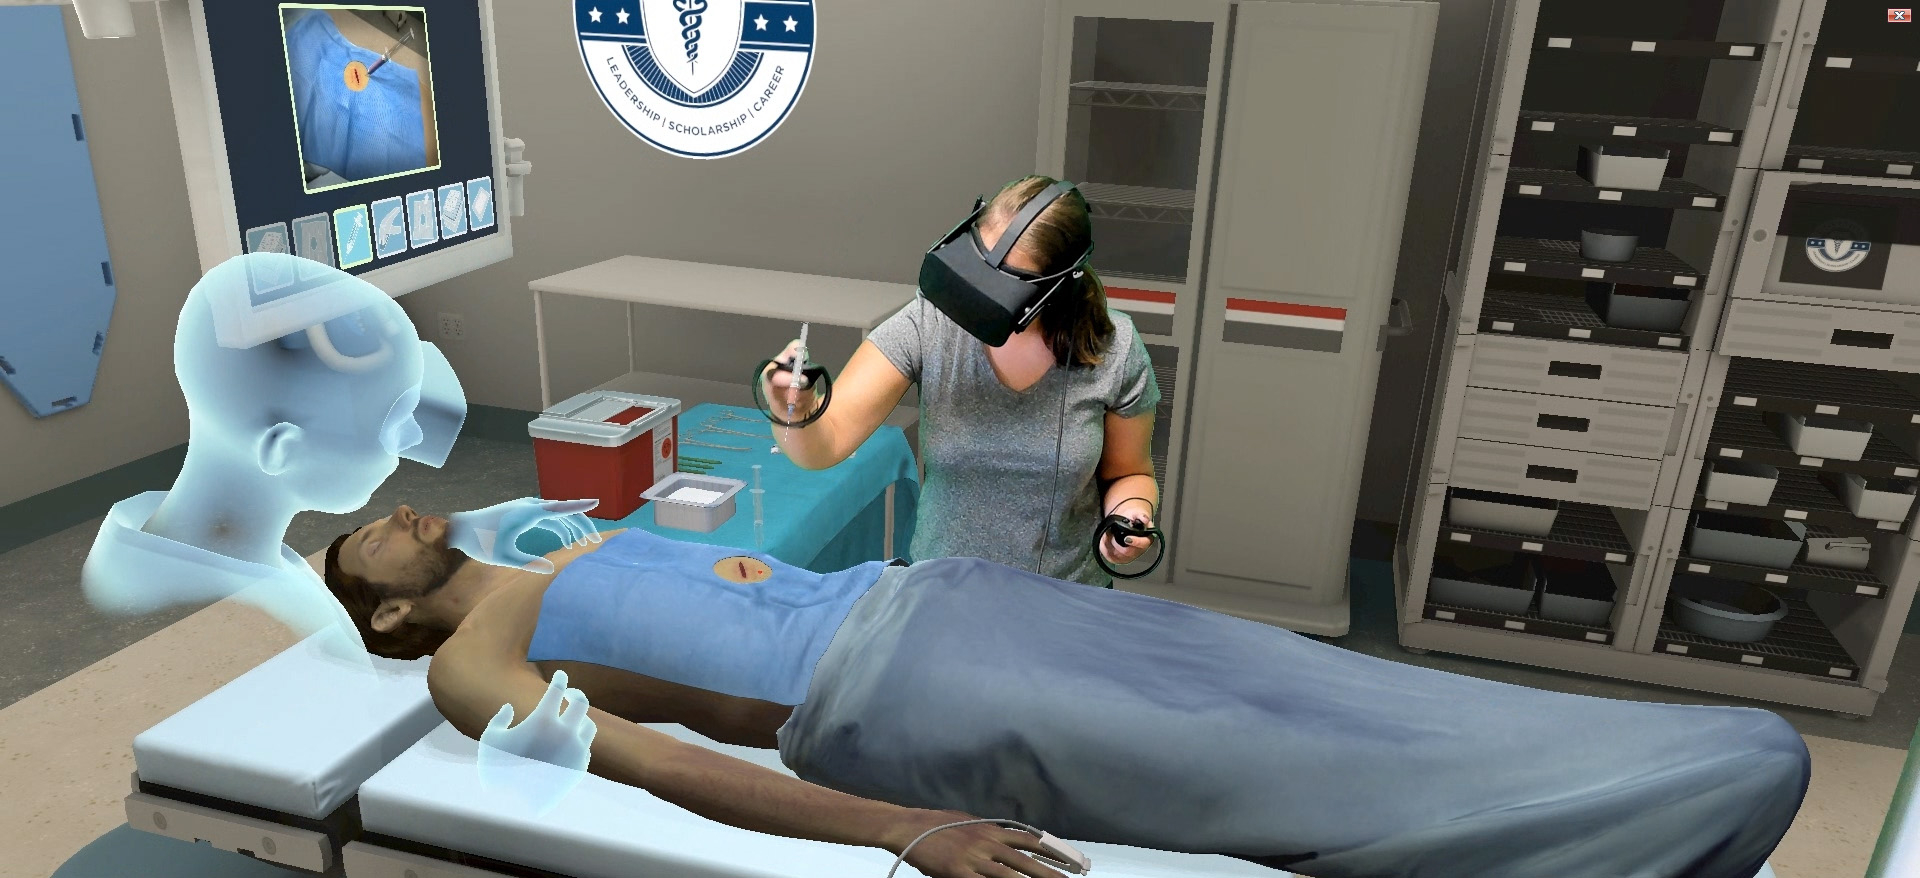
\includegraphics[width=.6\linewidth]{media/med_training_vr.jpg}
    \caption{A surgeon trains using VR \cite{med_train_vr}}
    \label{vr:med_train}
\end{figure}

\subsection{Analysis of a Standalone Headset: Oculus Quest}
A standalone, or all-in-one VR headset is a VR headset that is capable of storing games and
content on the device itself, and does all of its own processing without being connected
to a computer \cite{standalone_vr}. The Oculus Quest, one of the most popular
standalone VR headsets is shown below in Figure \ref{headsets:pictures}, along with
its controllers. This headset has a retail value of \$549.00 CAD \cite{quest_price}.

% Figure of headset
\begin{figure}[h]
    \centering
    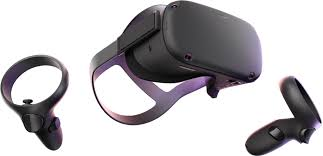
\includegraphics[width=.6\linewidth]{media/oculus_quest.jpg}
    \caption{Oculus Quest VR Headset \cite{quest_headset}}
    \label{headsets:pictures}
\end{figure}

Games and content are loaded onto the device wirelessly via a mobile phone app, 
and the headset can then be used anywhere to experience VR gameplay \cite{quest_features}. 
This device is meant for consumers who want to experience VR gaming, 
but do not already have an expensive gaming computer, or do not want 
to make that large investment.

\subsubsection{Hardware and Functionality}
The Oculus Quest runs on the Qualcomm Snapdragon 835 mobile system on chip (SoC) \cite{oculus_dev_page}.
This SoC is responsible for all processing and wireless connectivity on the headset. Some 
of the technical specifications of the Snapdragon 835 are shown
below in Table \ref{table:snapdragon}. In addition to the specifications listed in Table
\ref{table:snapdragon}, the Snapdragon 835 has hardware and sensors to support
cellular, Wi-Fi, Bluetooth, Near Field Communication (NFC), and location services
\cite{snapdragon_835}. The Snapdragon 835 is designed to offer powerful graphics
processing power in a low-power and low-footprint design, making it an appropriate
choice for a standalone VR headset.

% Snapdragon 835
\begin{table}[h]
    \centering
    \caption{Snapdragon 835 SoC Technical Specifications}
    \csvautotabular{data/quest_specs.csv} 
    \label{table:snapdragon} 
\end{table}

The Kryo 280 CPU implements the ARMv8-A 64-bit pipelined instruction set 
architecture \cite{kryo_arch}. It has eight cores, four of which can run up to
the maximum of 2.45 GHz and have a 2MB L2 cache, while the four slower cores have
a 1MB L2 cache, and the L1 caches are 64kB + 64kB \cite{snapdragon_cache}. The Adreno
540 GPU supports all of the most common graphics APIs, such as OpenGL, Vulkan,
OpenCL, and DirectX 12, allowing a wide support set for the visuals it can render \cite{snapdragon_835}.
The Snapdragon 835 chip offers all of this functionality in a low-power, low-footprint
design. In Figure \ref{fig:penny_835} the SoC is pictured next to an American penny for
scale.

\begin{figure}[h]
    \centering
    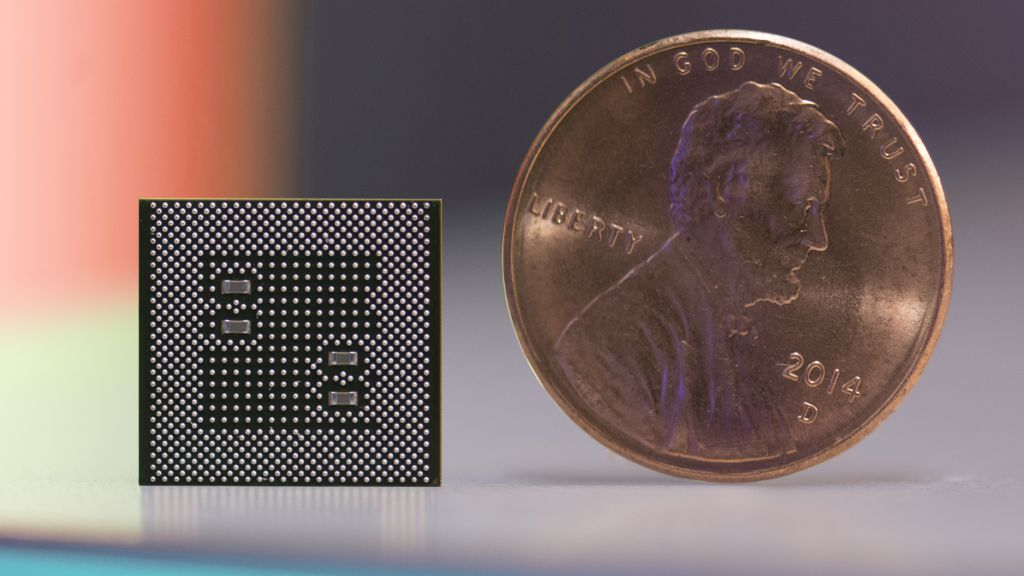
\includegraphics[width=.5\linewidth]{media/snapdragon_penny.jpg}
    \caption{Snapdragon 835 footprint compared to a penny \cite{penny_pic}}
    \label{fig:penny_835}
\end{figure}

The sensors onboard the Quest allow for six degrees of freedom (6DOF) in both the headset
and its controllers. This means that accurate tracking is provided for all three dimensions,
and orientation along those axes \cite{sixdof_defn}. The 6DOF tracking allows the player's
inputs to be as accurate as possible in the virtual world. The model of the Quest 
listed above for \$549 CAD comes with 64GB of internal storage, and 4GB of memory
\cite{quest_timemag}. The Snapdragon 835 SoC and these memory specifications
are very similar to that of a mobile phone. In fact, the Google Pixel 2 smartphone
uses the Snapdragon 835 chip, and comes with the same storage and memory
specifications \cite{quest_polygon}. The only difference is the Quest is
specialized to be a powerful graphics processing machine, while the Pixel 2
is meant to be a more general-purpose device, being a smartphone.

\subsubsection{Oculus Quest Summary}
Given the fact that the Oculus Quest is a standalone VR headset, and it contains
near identical specifications to a smartphone, it is appropriately priced close to
smartphone prices. This price allows the headset to be a good choice for an 
entry-level headset for consumers that want to experience VR without the 
large up-front cost of a high-performance computer being a barrier to entry.
Obviously, the VR experience will not be as clean on the Oculus Quest when compared
to VR headsets that connect to a computer (such as the Oculus Rift S), because processing
and rendering power of a desktop computer compared to that of smartphones is enormous,
but this is why the Quest is meant for entry-level consumers without these powerful
computers.